\subsection{Experiment 2 - Varying boundary conditions}
In this experiment we will examine the effect of having different boundary conditions along the boundary. We know when we define $c(p) = 0$ our solution will be a linear plane between going from the lower boundary condition to the upper boundary condition. We will now try to give 'nonsense' boundary conditions in the sense that our boundaries will now be tilted instead of uniform. The result can be seen in \autoref{linearrotated}.
\begin{figure}
	\centering
	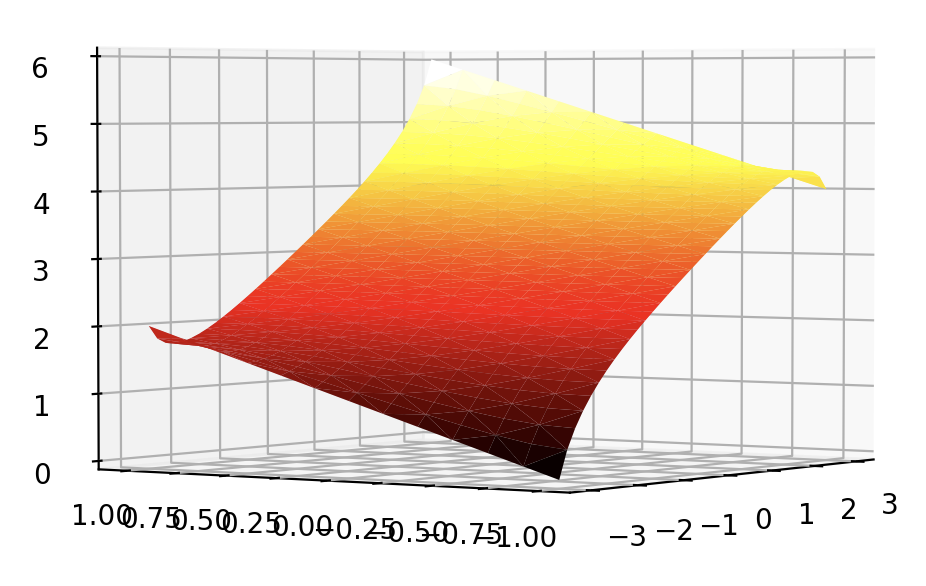
\includegraphics[width=\linewidth]{Materials/boundary}
	\caption{Linear 'rotated' boundary conditions.}
	\label{linearrotated}
\end{figure}
We here see the lower boundary values going linearly from 0 to 2 whereas the upper boundaries going linearly from 4 to 6. The resulting approximation looks a lot like the result when using uniform boundary conditions. In the middle the solution seems to be the same, and at the boundaries it seems the solutions has tried to 'adapt' to the 'rotated' boundary. This is in contrast to what we might have expected, namely the entire surface had rotated to match the new boundaries. We can now attempt to use some more random values at the boundaries to create a jagged boundary. The result can be seen in \autoref{jagged}.
 \begin{figure}
 	\centering
 	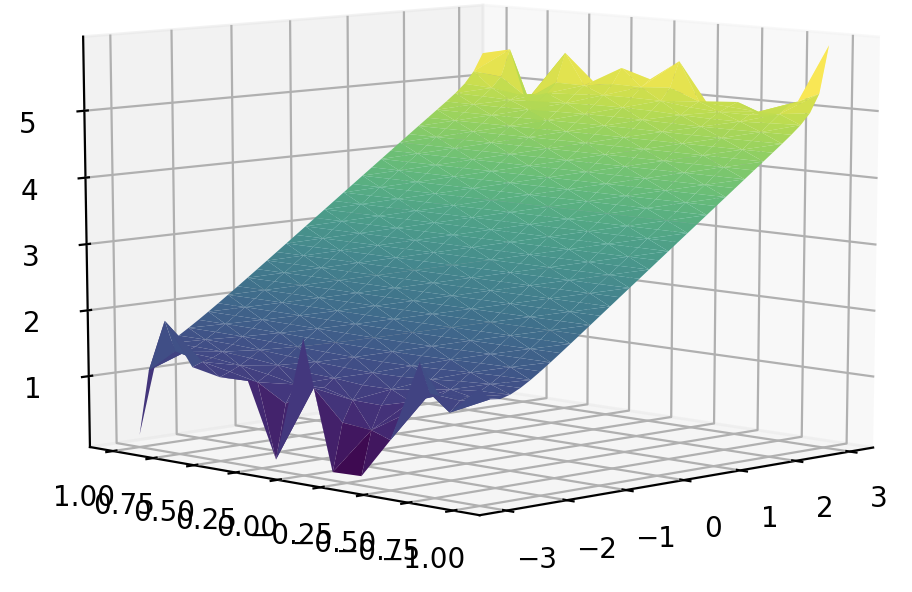
\includegraphics[width=\linewidth]{Materials/jagged}
 	\caption{Jagged boundary conditions.}
 	\label{jagged}
 \end{figure}
We here see almost the entire surface approximates the 'regular' solution with uniform boundary conditions and only barely changes due to the jagged boundaries.

\subsubsection{Discussion of results}
We end this experiment by concluding the approximations for the most part does not change as we change the boundaries, and rather than redefining the solution the boundary conditions gets incorporated into the solution.